\documentclass[a4paper,titlepage]{article}
\usepackage{graphicx}
\usepackage{subcaption}
\usepackage[default,oldstyle,scale=0.95]{opensans} %% Alternatively
%% use the option 'defaultsans' instead of 'default' to replace the
%% sans serif font only.
\usepackage[margin=1in]{geometry}

\usepackage[T1]{fontenc}
\usepackage{setspace}
\usepackage{fancyhdr}
\setlength{\headheight}{15.2pt}
\pagestyle{fancyplain}
\fancyhf{} % sets both header and footer to nothing
\renewcommand{\headrulewidth}{0pt}
\fancyfoot[L]{Lebanon Internet Report - 2020}
\fancyfoot[R]{\thepage}
\usepackage{xcolor,sectsty}

\definecolor{astral}{RGB}{46,116,181}
\subsectionfont{\color{astral}}
\sectionfont{\color{astral}}

%opening
\title{\color{astral}\Huge \bfseries Lebanon Internet Report}
\author{Maria Achkouty, Melissa Hussein, Youmna Bahout, and Samer Lahoud}

\onehalfspacing
\begin{document}

\maketitle

\begin{abstract}

\end{abstract}

\section{Introduction}
This report aims to describe the current state of Internet development in Lebanon and the surrounding countries. It offers an analysis of growth trends and Internet routing in the country.
We will discuss the use of the Internet across the country based on data from the International Telecom Union (ITU) portraying the evolution of penetration rate of the Internet in the MEA countries as well as mobile cellular and fixed broadband subscriptions. Then we will analyze addressing modes by touching upon LIR registered accounts to RIPE NCC determining the countries of origin of LIRs offering services in Lebanon.
Other parts of the report explore IPv4 holdings and the growth in the number of the prefixes in the Middle East which data was gathered from RIPE NCC’s website. We go into the exhaustion timeline of IPv4 then we deduct a potential growth in IPv6 from the observation of the data similarly collected.
Subsequently, we visualize with interactive graphs made using the distribution of IPv4 and IPv6 addresses by Lebanese autonomous systems taking away from it what autonomous systems have the biggest share of addresses.
Following this, our code will also allow us to view the results obtained from the RIPE database portraying autonomous systems’ evolution in Lebanon highlighting the different sectors of activity from ISPs to banks to universities ...
We then study internal routing in the country with the statistics we got from performing traceroutes between online Lebanese probes.
Finally, we highlight Lebanon’s international connectivity with an interactive Sankey diagram illustrating which networks provide BGP route announcements.
This would be the first detailed report done for Lebanon. We hope to provide technical insight and make the data available to the local community and decision makers. Hence, supporting the internet development in the country.

The report focuses on what we can observe and measure from RIPE NCC services and measurement infrastructure in the region. With a greater number of data collection points and more information sharing between stakeholders in the region, we would be able to provide an even more detailed and complete analysis of the situation in the future. To this end, the report also contains information on how all stakeholders can help support further analysis.

\section{Internet Use Across the Country}
The percentage of people using the Internet across the Middle Eastern countries has been increasing quite steadily in most of them and at a rapid rate in some others (i.e UAE, Lebanon). Figure 1 shows that Lebanon places in the middle.
In 2001, the penetration rate was extremely low (less than 10\%) and began to increase rapidly between 2008 and 2013. However, this evolution slowed down around 2014. This may be due to the government cutting off access to mobile Internet services in Arsal in the northeast of Lebanon in 2014 for political reasons. This shutdown lasted around three years. Moreover, in July 2015, there was a breakdown of several thousand telephone and Internet lines in Beirut due to the waste incineration.
In 2017, Lebanon’s penetration rate reached 78% which gives room for future growth and investment.

\begin{figure}
    \centering
    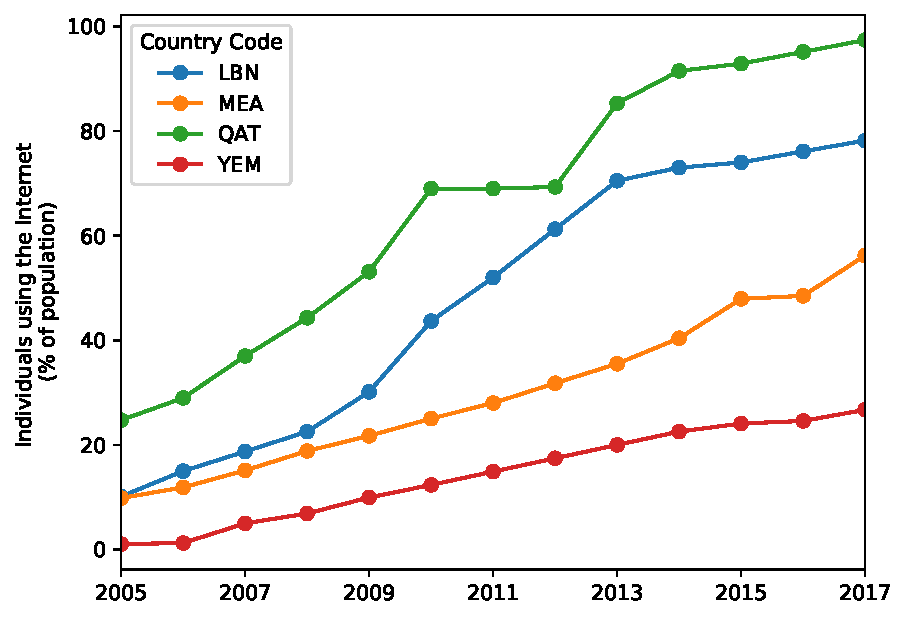
\includegraphics[width=0.75\linewidth]{../output/internet-users.pdf}
    \caption{Evolution of the percentage of population using the Internet in selected countries in the Middle East. The figures displayed here are obtained from ITU data on Internet users by country and World Bank population data [the ITU does not as yet provide data on Lebanon past 2017].}
\end{figure}

\begin{figure}
    \centering
    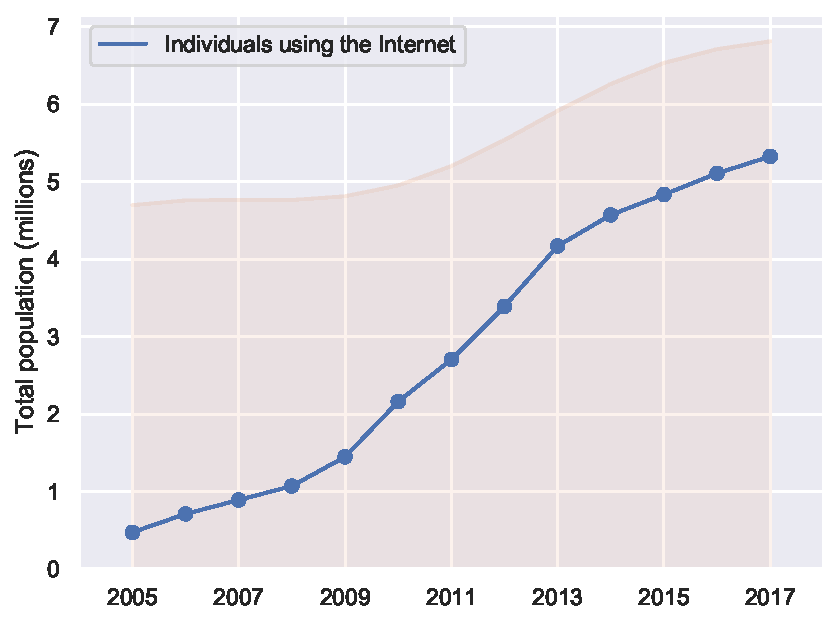
\includegraphics[width=0.75\linewidth]{../output/population-internet-lbn.pdf}
    \caption{test}
\end{figure}

\begin{figure}
    \centering
    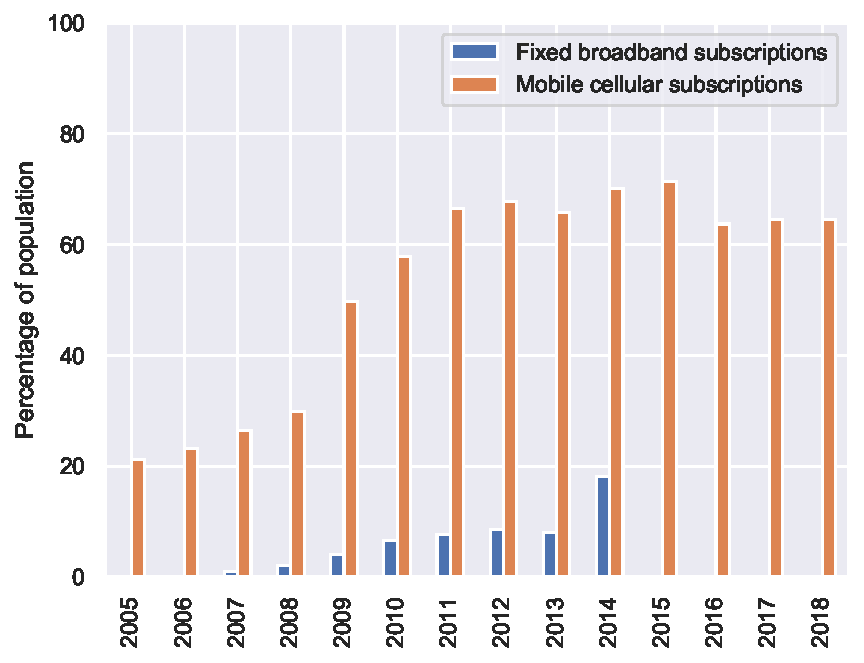
\includegraphics[width=0.75\linewidth]{../output/aggregate-lbs-users.pdf}
    \caption{test}
\end{figure}

\begin{figure}
    \centering
    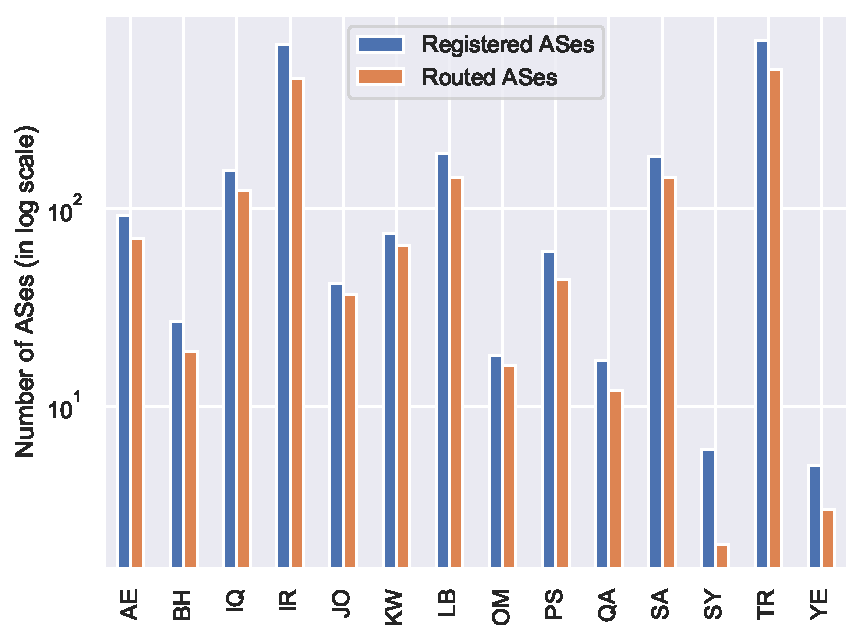
\includegraphics[width=0.75\linewidth]{../output/as-stat.pdf}
    \caption{test}
\end{figure}

% \begin{figure}
%     \centering
%     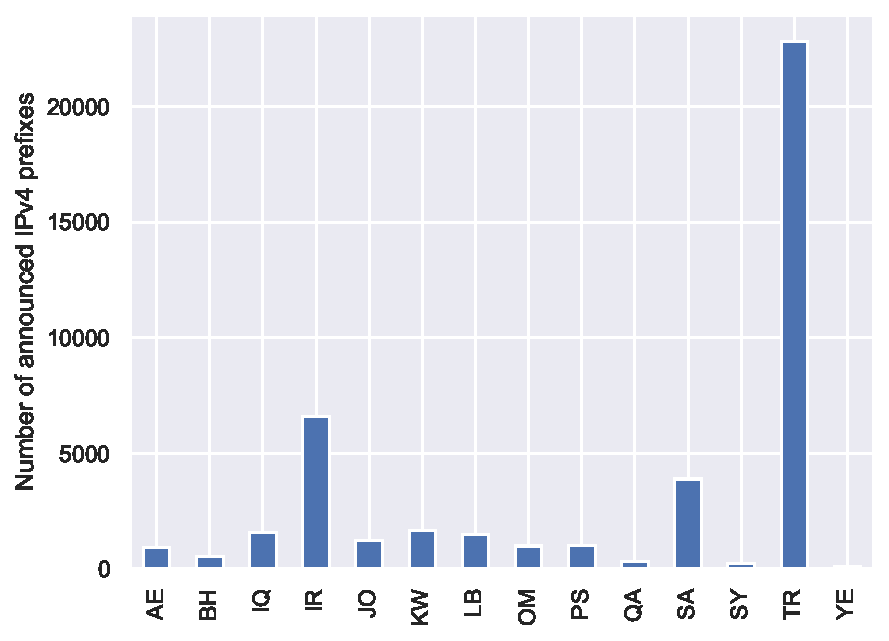
\includegraphics[width=0.75\linewidth]{../output/prefix-v4.pdf}
%     \caption{test}
% \end{figure}

% \begin{figure}
%     \centering
%     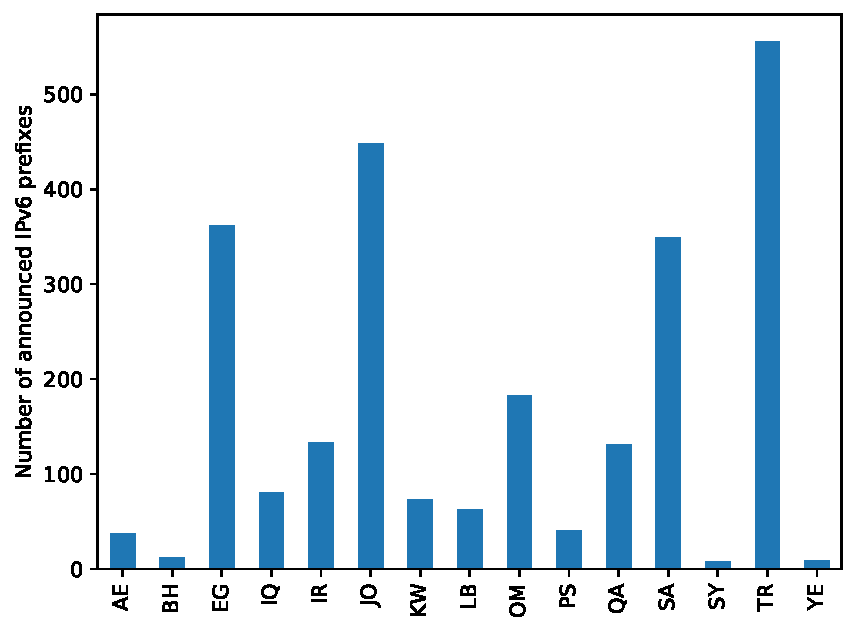
\includegraphics[width=0.75\linewidth]{../output/prefix-v6.pdf}
%     \caption{test}
% \end{figure}

\begin{figure}
    \centering
    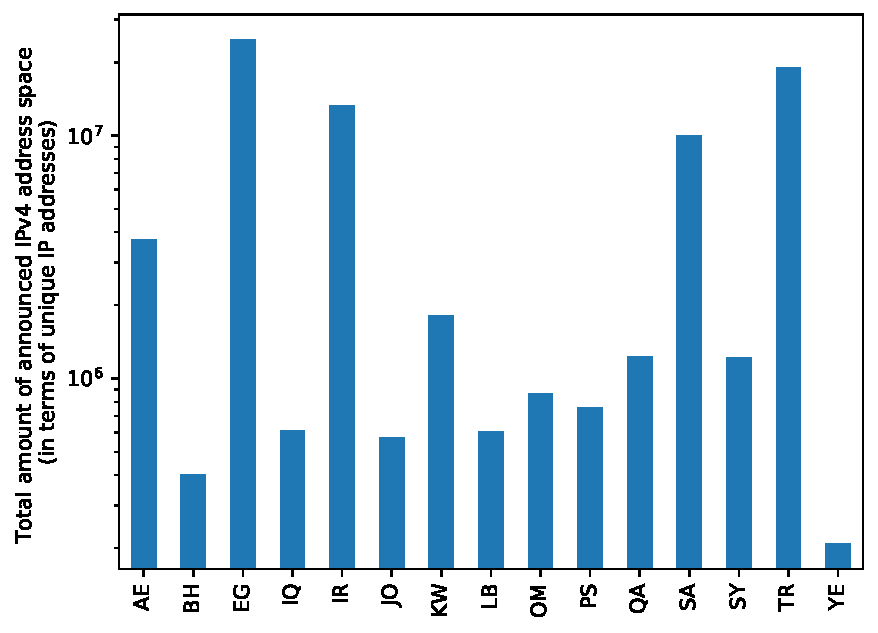
\includegraphics[width=0.75\linewidth]{../output/ips-v4.pdf}
    \caption{test}
\end{figure}

\begin{figure}
    \centering
    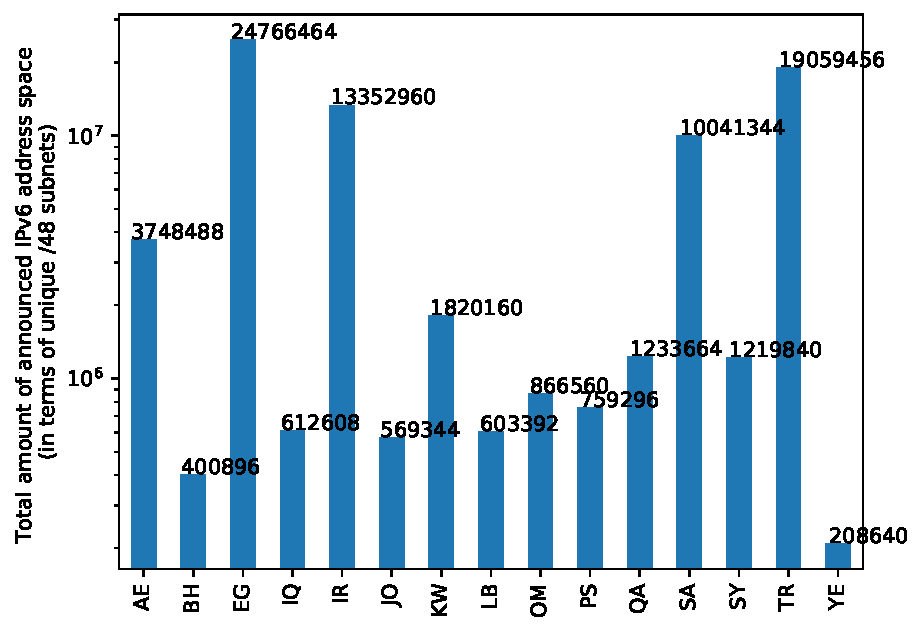
\includegraphics[width=0.75\linewidth]{../output/48s-v6.pdf}
    \caption{test}
\end{figure}

\begin{figure}
    \centering
    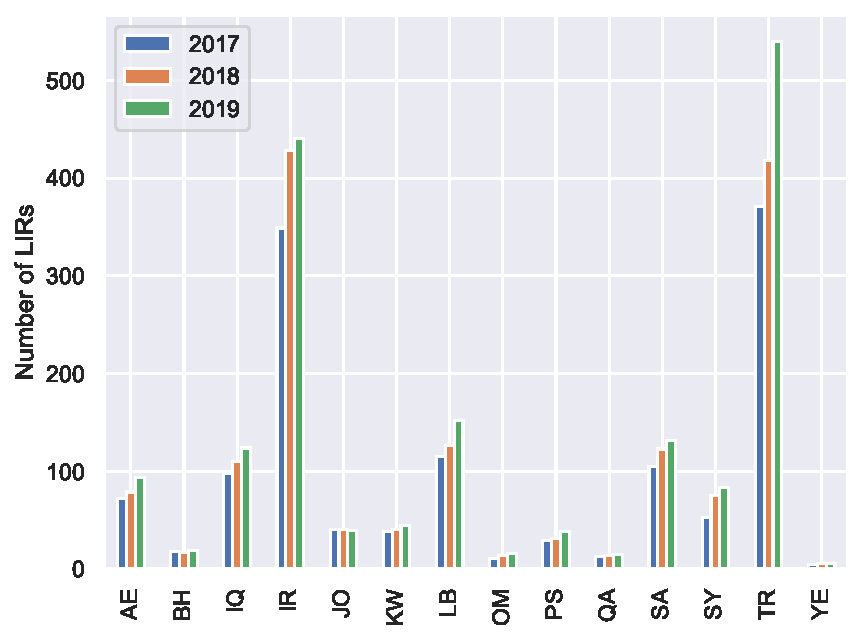
\includegraphics[width=0.75\linewidth]{../output/lir.pdf}
    \caption{test}
\end{figure}

\begin{figure}
    \centering
    \subcaptionbox{Frequency bands.\label{fig:perc-band-evo}}
    {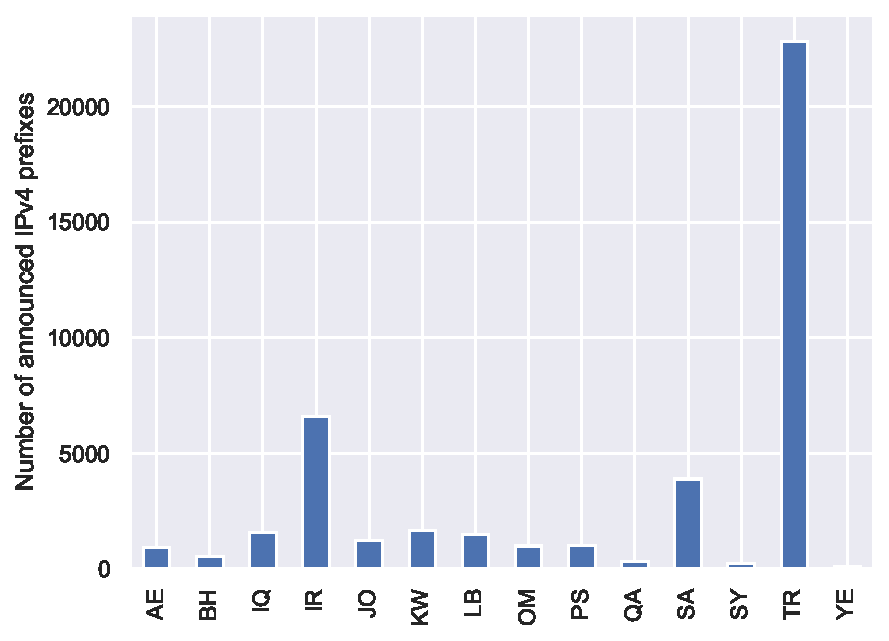
\includegraphics[width=0.45\linewidth]{../output/prefix-v4.pdf}}
    \subcaptionbox{Mobile technologies.\label{fig:perc-techno-evo}}
    {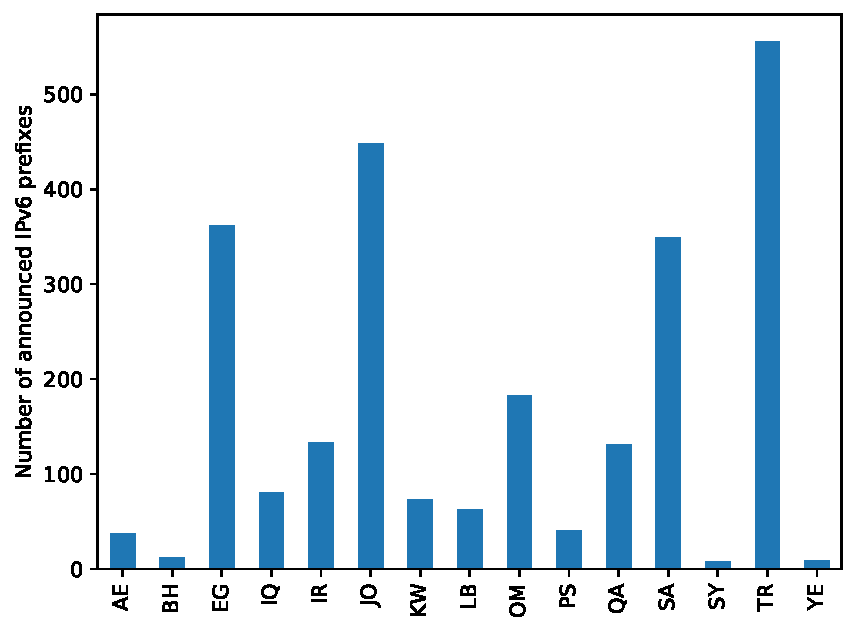
\includegraphics[width=0.45\linewidth]{../output/prefix-v6.pdf}}
    \caption{Evolution of the spectrum utilization in the city of Rennes in France.
    \label{fig:perc-antenna-evo}
    }
\end{figure}

\end{document}